\begin{figure*}[h]                                                           
 \includegraphics[width=\linewidth]{./media/images/chart}%
  \small{\textsc{\\ Planning your adventure} doesn't have to be a slog\textemdash
    here are some tools to help (Photo:
    \href{https://en.wikipedia.org/wiki/File:Pedro_Reinel_1504.jpg}{\textsc{Bayerische Staatsbibliothek, Munchen).}}}
  \label{fig:planning}%                                                 
\end{figure*}                                                                
\begin{quotation} 
\noindent\color{Sepia}{\scriptsize{\textit{\textbf{“Reality is merely an illusion, albeit a very persistent one..” }}}}\\[2mm]
   \hfill\color{Sepia}{\scriptsize{\textendash Albert Einstein}}
\end{quotation} 

\lettrine[lines=3]{\color{BrickRed}S}{\enspace o} you have an idea for your work of Interactive Fiction. You've mulled the idea
around for some time\textemdash now it's time to start putting your thoughts on
paper (or screen, as it were) but where to start?
\marginpar{\vspace{-2mm}
  \tiny{\textit{Ready, set, go!}}
}

There is no One Way to build a work of IF. Like authorship itself, some writers
like to plan their work ahead of time. Others like to simply spring their writing
spontaneously. Still other authors like to work between a combination of the two.
\marginpar{
  \tiny{\textit{Planning is the key but it's better feeling unconstrained about
      the order of execution}}
}
Where IF differs from traditional authorship is the necessity for at least some
degree of planning. There are many methods for sketching out your work and I
make no constraints for the order by which you choose to build your world model.
You will likely find yourself iterating between the various layers of your work.
There is no need (and I would argue not as effective) to complete one layer
before beginning the next.

Simply by necessity of categorizing the craft of IF I offer the following broad
layers for producing quality work.

\section{physical world layer}
%cover image credit: https://en.wikipedia.org/wiki/File:CMMI_Project_Planning_%E2%80%93_Process-data_model.png
Your overall plot in mind probably lends itself to a setting. In the case of
\textit{The Acropolis} the setting is obvious\textemdash oddly enough, the
Acropolis itself. If you're new to writing IF you will give yourself a leg up on
finishing your product by taking inspiration from a physical location.
\marginnote{
 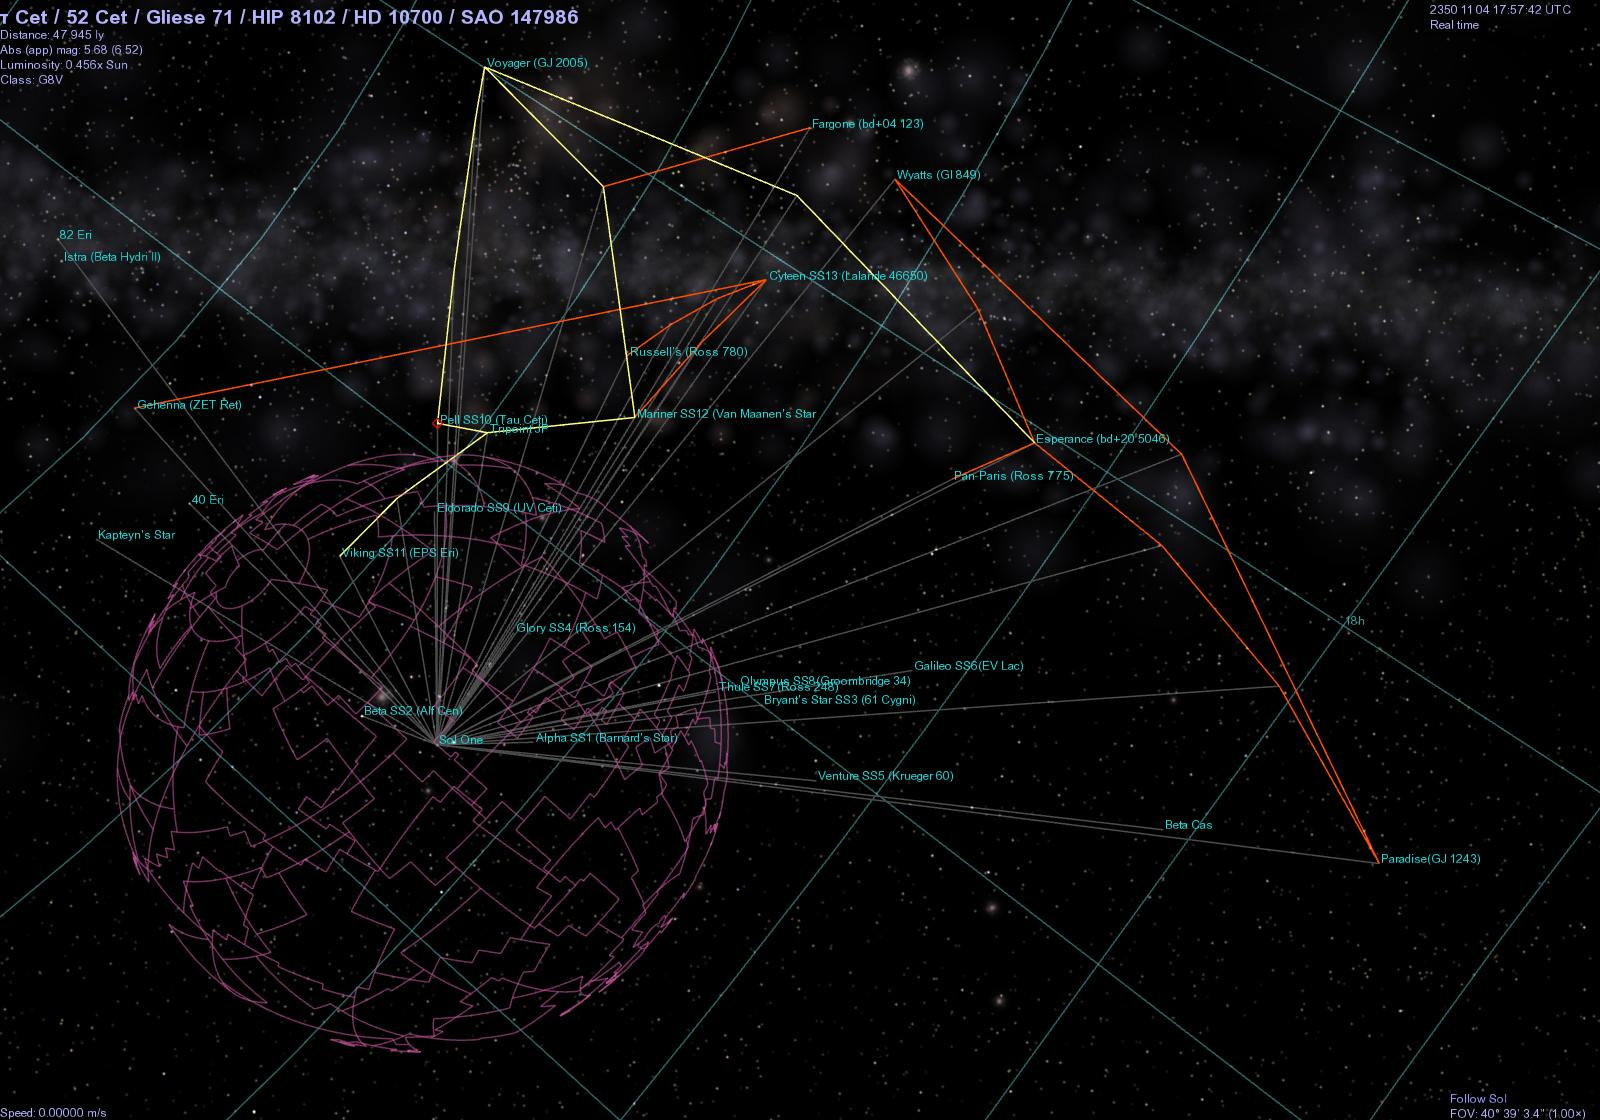
\includegraphics[width=\linewidth]{./media/images/star_map}%
  \tiny{\textit{\\ There exists virtually no end of maps you can use to inspire your work, including star maps (Photo:
    \href{https://www.classe.cornell.edu/~seb/celestia/pell/images/alliance-union-trade-routes.jpg}{\textsc{celestia
        screen capture).}}}
  \label{fig:starmap}%
  }
}
You also serve yourself as your work will ``feel'' real, similar to the way the venerable \textit{Colossal Caves Adventure} is revered in no small part because it is based on a real cave. The reader finds himself immersed in
his environment because the work \textit{is} crafted from a real location, free from contrivances.

\begin{figure*}[h]                                                           
 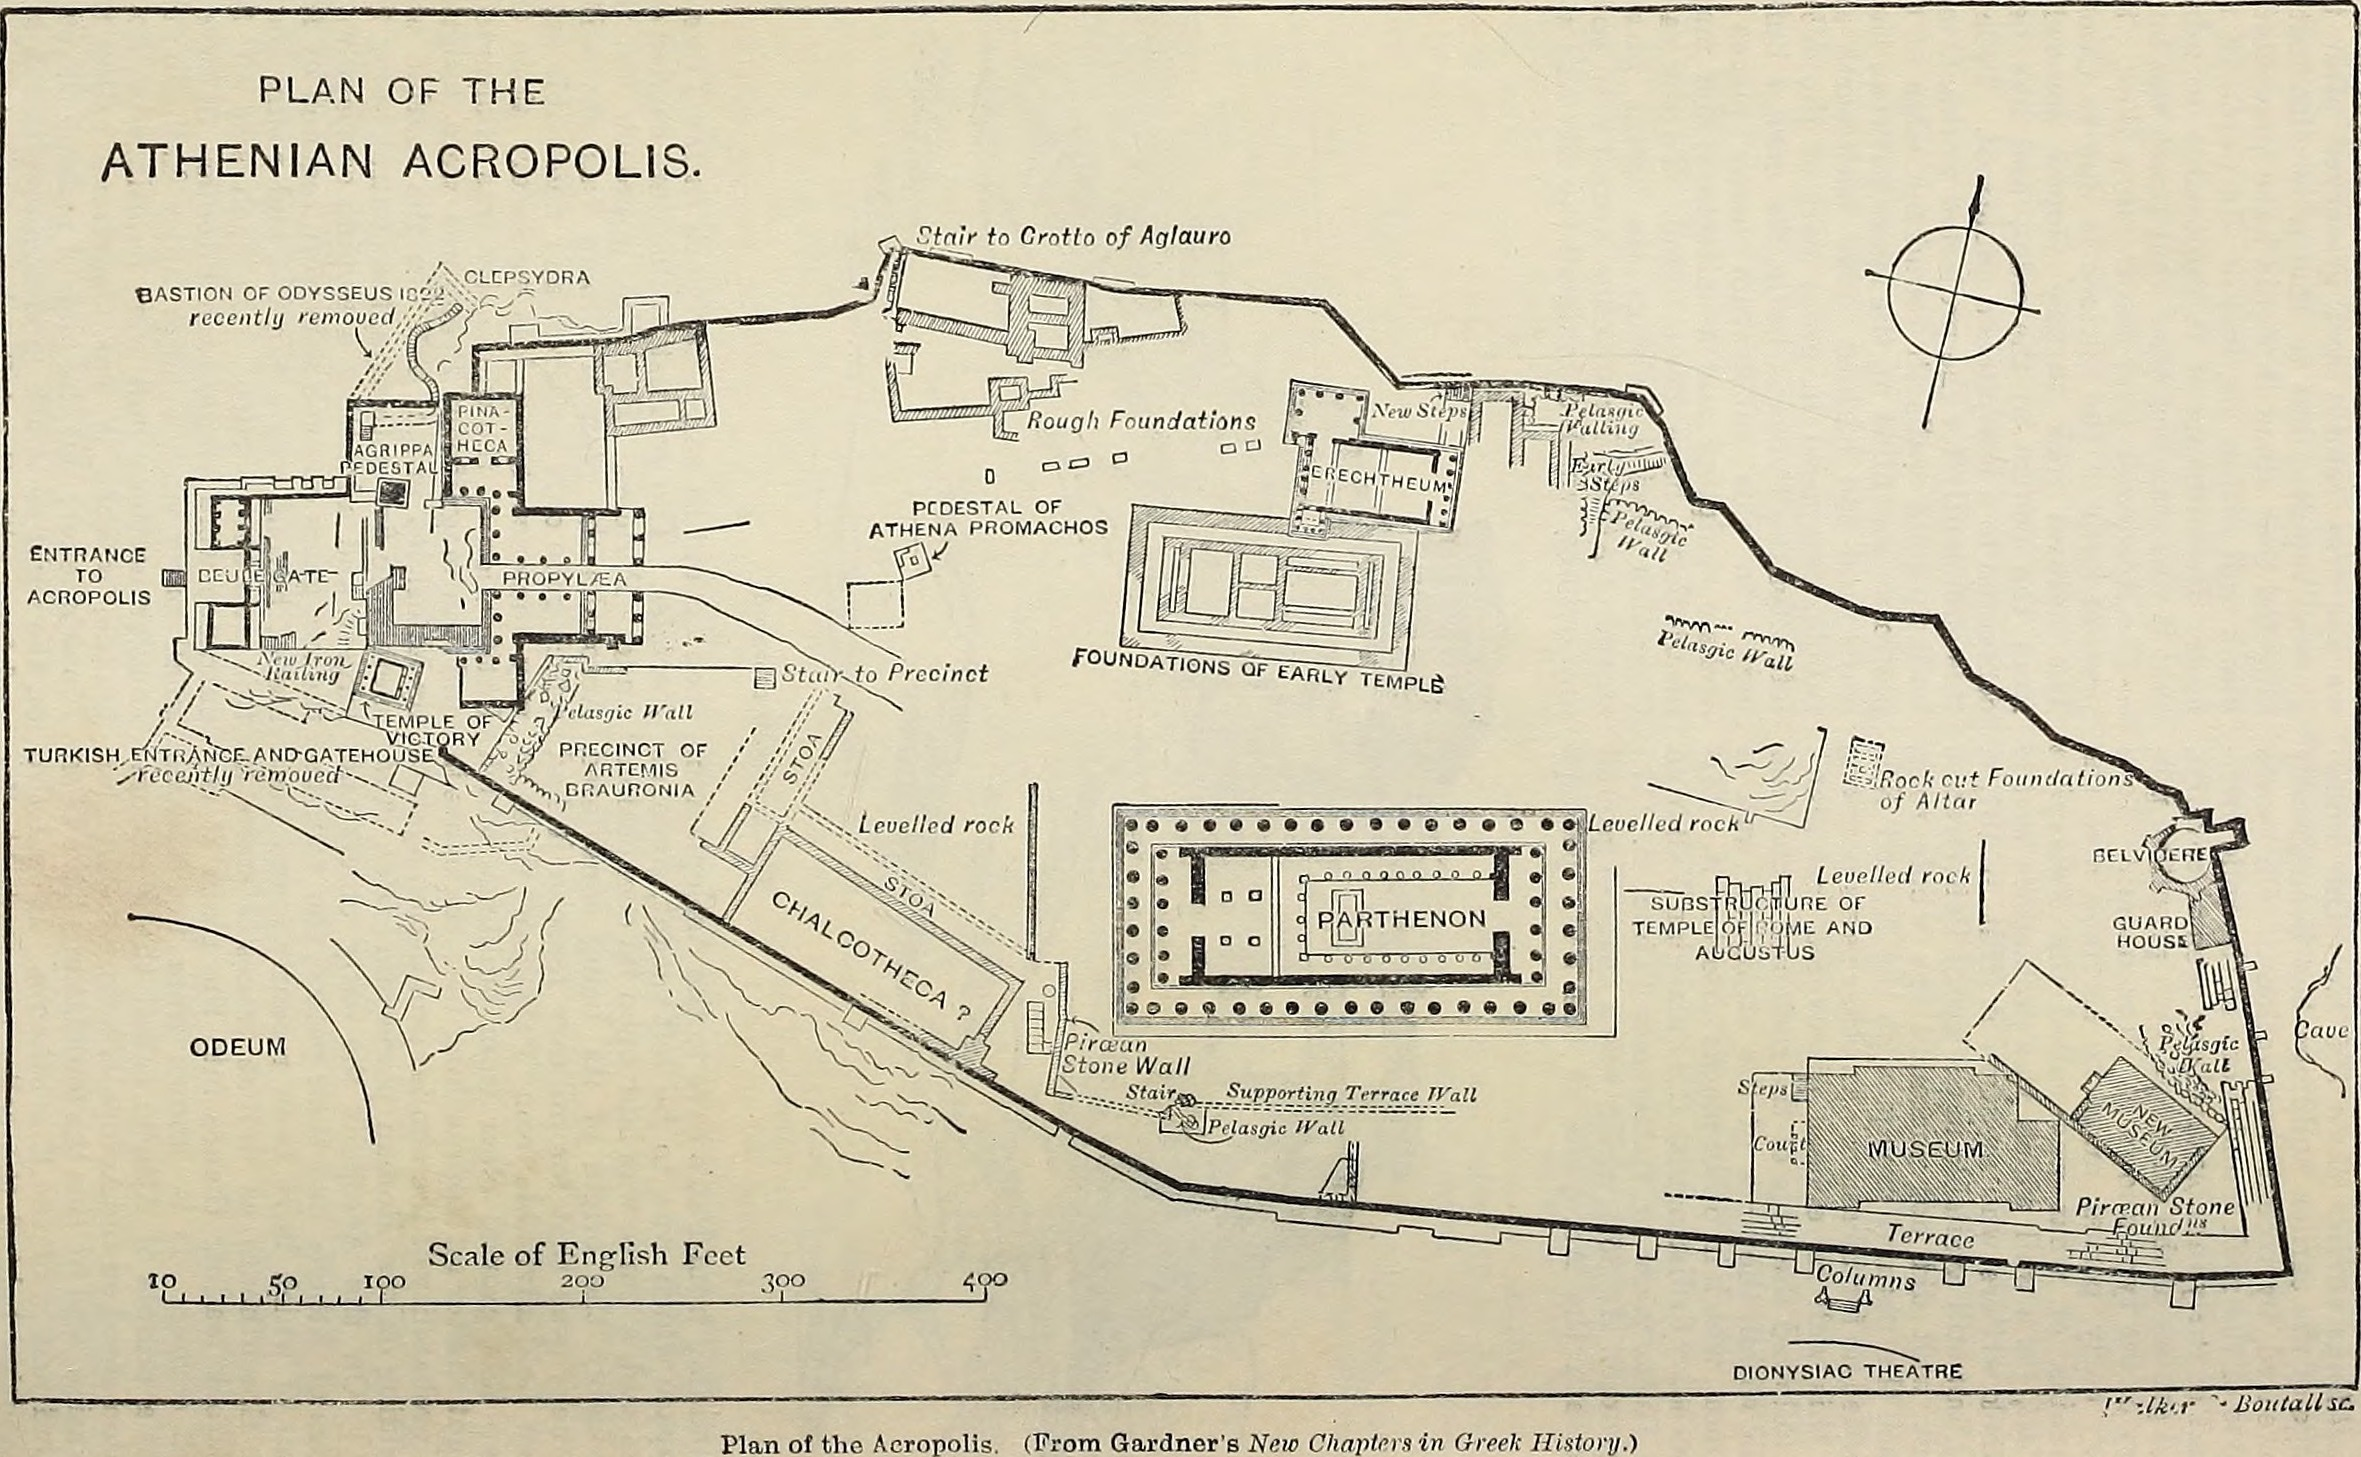
\includegraphics[width=\linewidth]{./media/images/acropolis_map}%
  \small{\textsc{\\ Real maps often} provide an effective source of inspiration (Photo:
    \href{https://commons.wikimedia.org/wiki/File:Plan_of_the_Athenian_Acropolis.jpg}{\textsc{A classical dictionary of Greek and Roman biography).}}}
  \label{fig:planning}%
\end{figure*}
A helpful method is to download a map and overlay your IF's map concept over that by

\reversemarginpar
\marginpar{\vspace{8mm}
  \tiny{\textit{Drawing inspiration and templating from real\textendash world
      source material.}}
}
drawing boxes over each location with connectors in\textendash between.
\textit{Inkscape}'s connector tool is effective for this as it gives you freedom
to place your locations wherever you like while taking care of the connector
details.


If you prefer a templated approach\textemdash one that will build a world model
for you after you've finished your map\textemdash
\href{http://ggarra13.github.io/ifmapper/en/}{\textsc{if mapper}} and
\href{https://trizbort.genstein.net/#overview}{\textsc{trizbort}} are two utilities to do
this. If you prefer a programmatic approach,
\href{https://ifm.readthedocs.io/en/latest/}{\textsc{ifm}} lets you create a map from a
text file. \href{https://github.com/dustinlacewell/t3sketch}{\textsc{t3sketch}} offers a
complete templating system for \textsc{tads3} (including build tools) to lay
down your world model (Hint: use the included xml file in the respository
\texttt{\tiny{t3sketch/example/living\_quarters.xml}} to get started).

\subsection{composing the scene}
You may find
\reversemarginpar
\marginnote{\tiny{\textit{Visiting a location and writing everything
      about it inspires}}}
 yourself in a place where you've mapped your story (at least
partially) and find yourself with a myriad of empty location boxes needing a
description. One method I 'stole' from the excellent
\href{https://www.amazon.com/Travel-Writing-World-Sell-Story/dp/1582973814}{travel
writing: see the world. sell the story} book is to physically visit a location
with your notebook and simply, ``write like hell.'' Capture everything you're
experiencing in this location as scribbles\textemdash just get it all down. 
\normalmarginpar
\marginnote{
  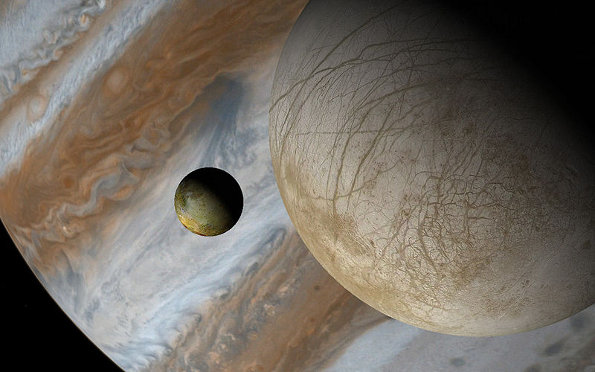
\includegraphics[width=\linewidth]{./media/images/celestia}
  \tiny{\textit{Celestia's ``free range'' space exploration system
      means you can accurately plot a universe for your work of Science Fiction (Photo:
      {\href{https://www.cyberciti.biz/tips/celestia-astronomy-linux-program.html}{
          Vivek Gite, nixCraft}})}}
  }
Record the sights, both local and distant, the smells, the sounds, etc. Your
location needn't necessarily be one similar to the locations in your work of IF
as you're almost certain to draw inspiration from your ``fast and furious''
writing on location.
\reversemarginpar
\marginnote{\tiny{\textit{Text summarizers are helpful for quickly drafting locations}}}
Another good way to fill in the boxes is to summarize works of text found on the
Internet that resemble your location with a natural language summerizing tool
like \href{https://github.com/miso-belica/sumy}{\textsc{sumy}}. Simply point
to your location description's \textsc{url} and let it generate a few
sentences about your location. Here's an example of the summarizer pointed to a
description of the Parthenon:

\begin{quote}
  \small{
\noindent \textbf{\$ sumy lex-rank --length=10 --url https://www.ancient.eu/parthenon/}

\noindent The magnificent temple on the Acropolis of Athens, known as the Parthenon, was built between 447 and 432 BCE in the Age of Pericles, and it was dedicated to the city ’s patron deity Athena.

From the 4th century BCE the whole building acquired the name Parthenon. The Parthenon would become the largest Doric Greek temple, although it was innovative in that it mixed the two architectural styles of Doric and the newer Ionic.

It was entered through large wooden doors embellished with decorations in bronze, ivory, and gold. The temple was unprecedented in both the quantity and quality of architectural sculpture used to decorate it.

The pediments of the temple measured 28.55 m in length with a maximum height of 3.45 m at their centre.

Many of the metopes on the other sides of the building were deliberately damaged and figures in the central part of the east pediment were removed.
} %end small
\end{quote}
\noindent Not bad. You've now a foothold by which to base your descriptions;
``slice and dice'' your summary to suit.

\section{a picture worth a thousand words}
Now we've mapped a framework for our world using a map tool, and used a summarizer
for each locations' description let's suppose we'd like to add images for some or all
of our locations.
  \marginpar{
    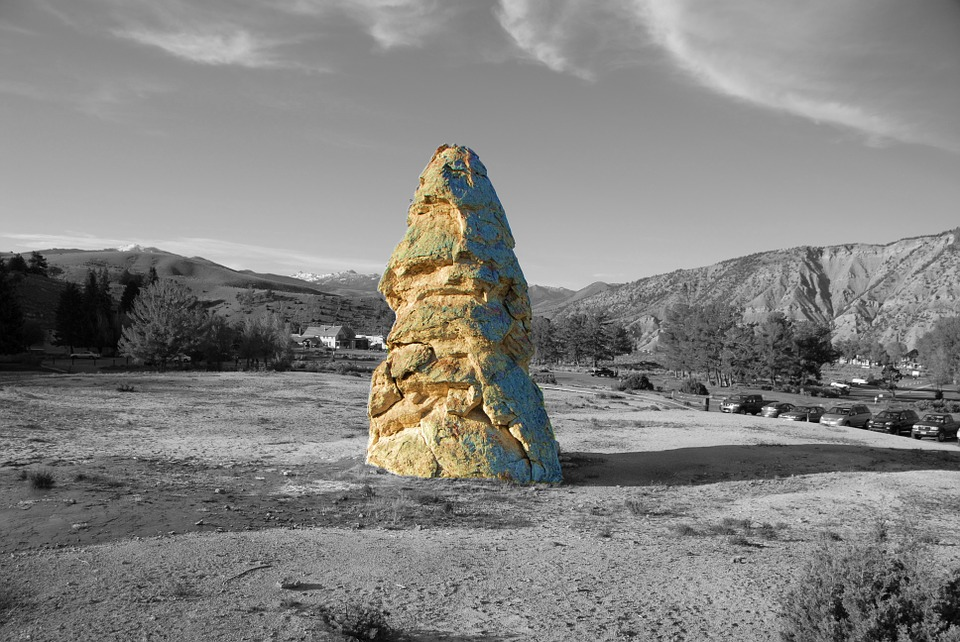
\includegraphics[width=\linewidth]{media/images/artistic_scenery}%
  \tiny{\textsc{\\ An artistic means} of capturing your readers' attention by the tasteful use of color on black\textendash and\textendash white (Photo: \href{https://pixabay.com/en/artistic-scenery-black-and-white-60871/}{\textsc{Pixabay: ``Steppinstars'').}}}
} %end marginpar
\begin{figure*}[h]                                                           
  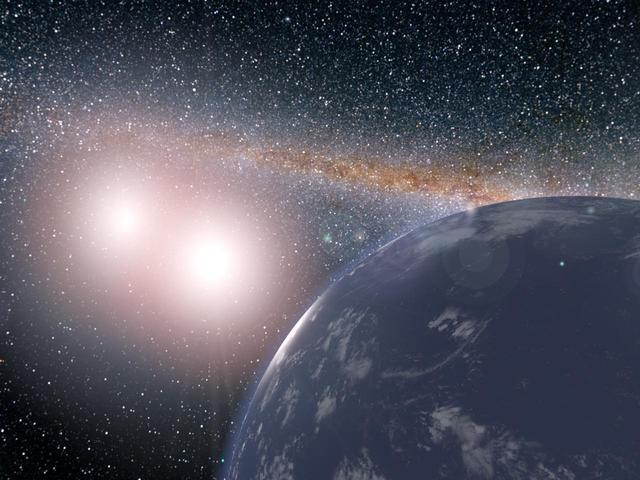
\includegraphics[width=\textwidth]{./media/images/exoplanet}
  \small{\textsc{Imagine your interlocutor as} the first to discover
      organic molecules with the help of freely available NASA images (Photo:
      \href{https://images.nasa.gov/details-PIA21470.html}{\textsc{nasa/jpl-caltech}})}
  \label{fig:nasa}
\end{figure*}

Obviously, pointing a search engine looking for appropriately licensed images
will do some of the job, and there are plenty of free resources for you to
include in your work. \href{https://pixabay.com/en/photos/}{\textsc{pixabay}},
\href{https://en.wikipedia.org/wiki/Wikipedia:Images}{\textsc{wikimedia}}, and
\href{https://pikwizard.com/}{\textsc{pikiwizard}} are all available to name a
few. Eric Matyas, by the way, offers a wide range of
\href{https://soundimage.org/}{\textsc{images and sound e{ff}ects}} available for
\textsc{if} authors; you need only provide the appropriate attribution for his work.

\subsection{blender}
\marginnote{
  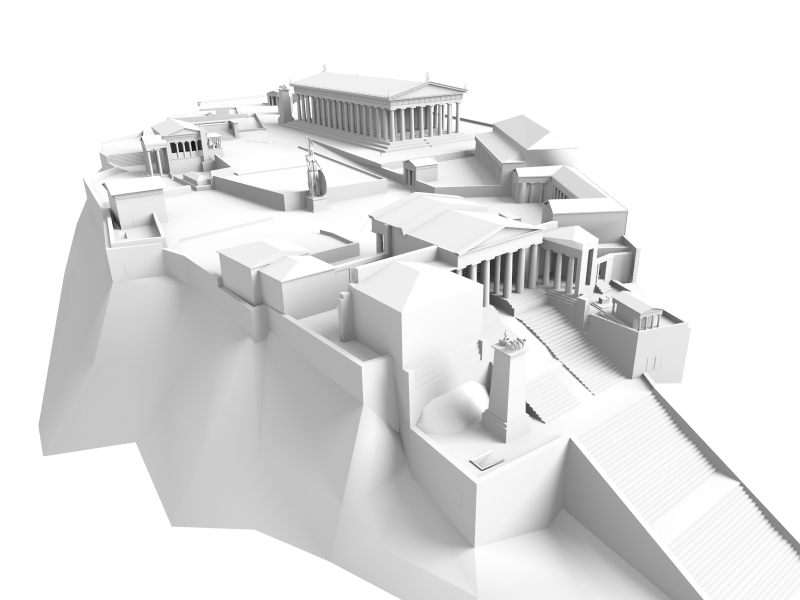
\includegraphics[width=\linewidth]{./media/images/acropolis_model}
  \tiny{\textsc{A 3D Model} \textit{of the Acropolis is free for download and use (Photo: {\href{https://www.blendernation.com/2012/11/30/model-download-acropolis-of-athens-165ad/}{Sebastian Kiersz}})}}
  }
\noindent Having a free, full\textendash fledged 3D modeler is tough to beat for giving
your readers a graphical way to orient themselves in your world model.
Complete agency extends as far as your imagination. It's not hard to imagine a
super\textendash imposed compass rose on the floor of each location to further
ease the interlocutor's navigation through your world. In the case of \textit{Acropolis} a \href{https://www.blendernation.com/2012/11/30/model-download-acropolis-of-athens-165ad/}{\textsc{ready\textendash made model exists}}.
\subsection{flight simulator}
You can map out entire outdoor spaces using
\marginnote{
  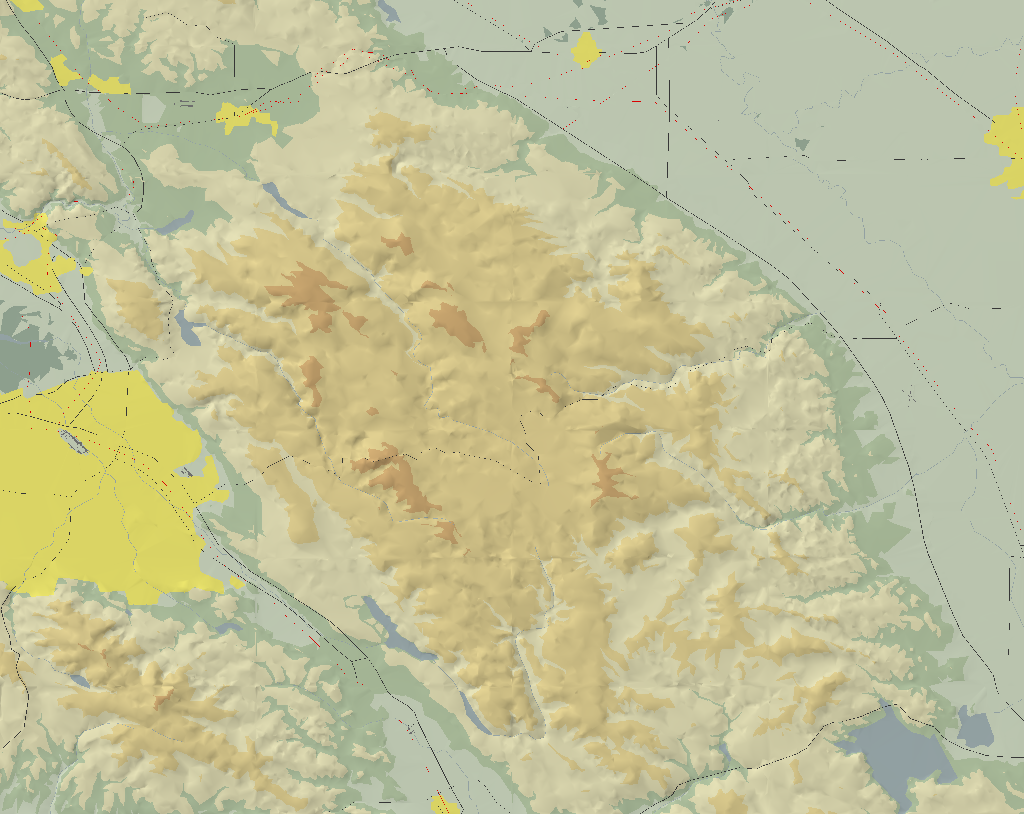
\includegraphics[width=\linewidth]{./media/images/fg_map}
  \tiny{\textit{FlightGear's map modelling software makes making good\textendash
      looking maps easy (Photo:
      \href{http://geoffmclane.com/fg/atlas-07.htm}{\textsc{geoff mclane}}})}
}
\href{http://home.flightgear.org/}{\textsc{flightgear}}'s mapping and view
options. Flightgear is quality open source flight simulator that is available
for free download. You can use Flightgear to map out accurate \textsc{gis}
experiences or as an inspiration to an environment of your creation.
\begin{figure*}[h]                                                           
 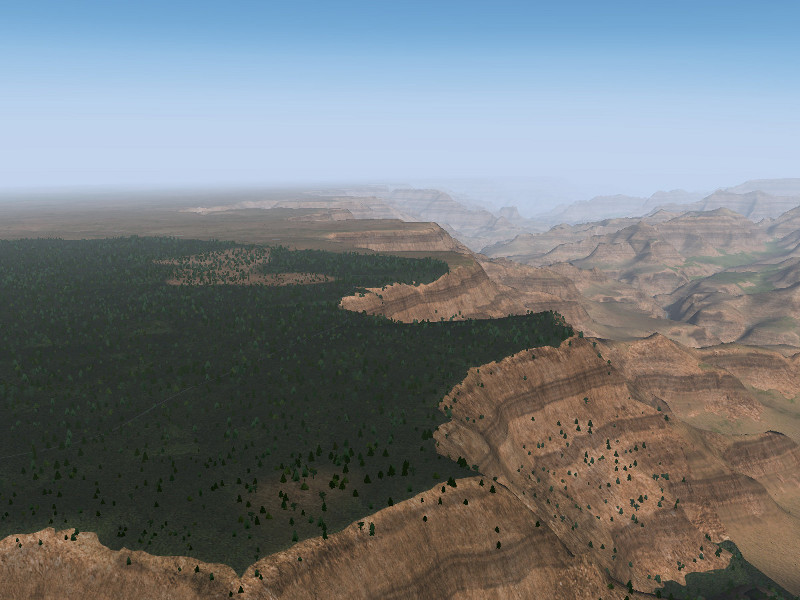
\includegraphics[width=\linewidth]{./media/images/fg_scenery}%
  \small{\textsc{\\ FlightGear offers detailed }\,\& stunning views of natural
    terrain (Photo:
    \href{http://www.flightgear.org/wp-content/uploads/2014/09/dds-regional-ALS.jpg}{\textsc{Flightgear
        project).}}}
  \label{fig:fg_scenery}%                                                 
\end{figure*}                                                                
First, use the \href{https://www.maps.ie/coordinates.html}{\textsc{a map tool supporting latitude/longitude coordinates}} to plot the points you want to
describe. Then use FlightGear's ``\textsc{ufo} mode'' to place your location precisely where you want
it. You can use either a screenshot tool or FlightGear's built\textendash in
tool to capture the scene. If you're really ambitious you can capture a scene
for each compass direction should the interlocutor type a look directive with a
specific direction like \texttt{\small{>\,look east}}.

\marginnote{
  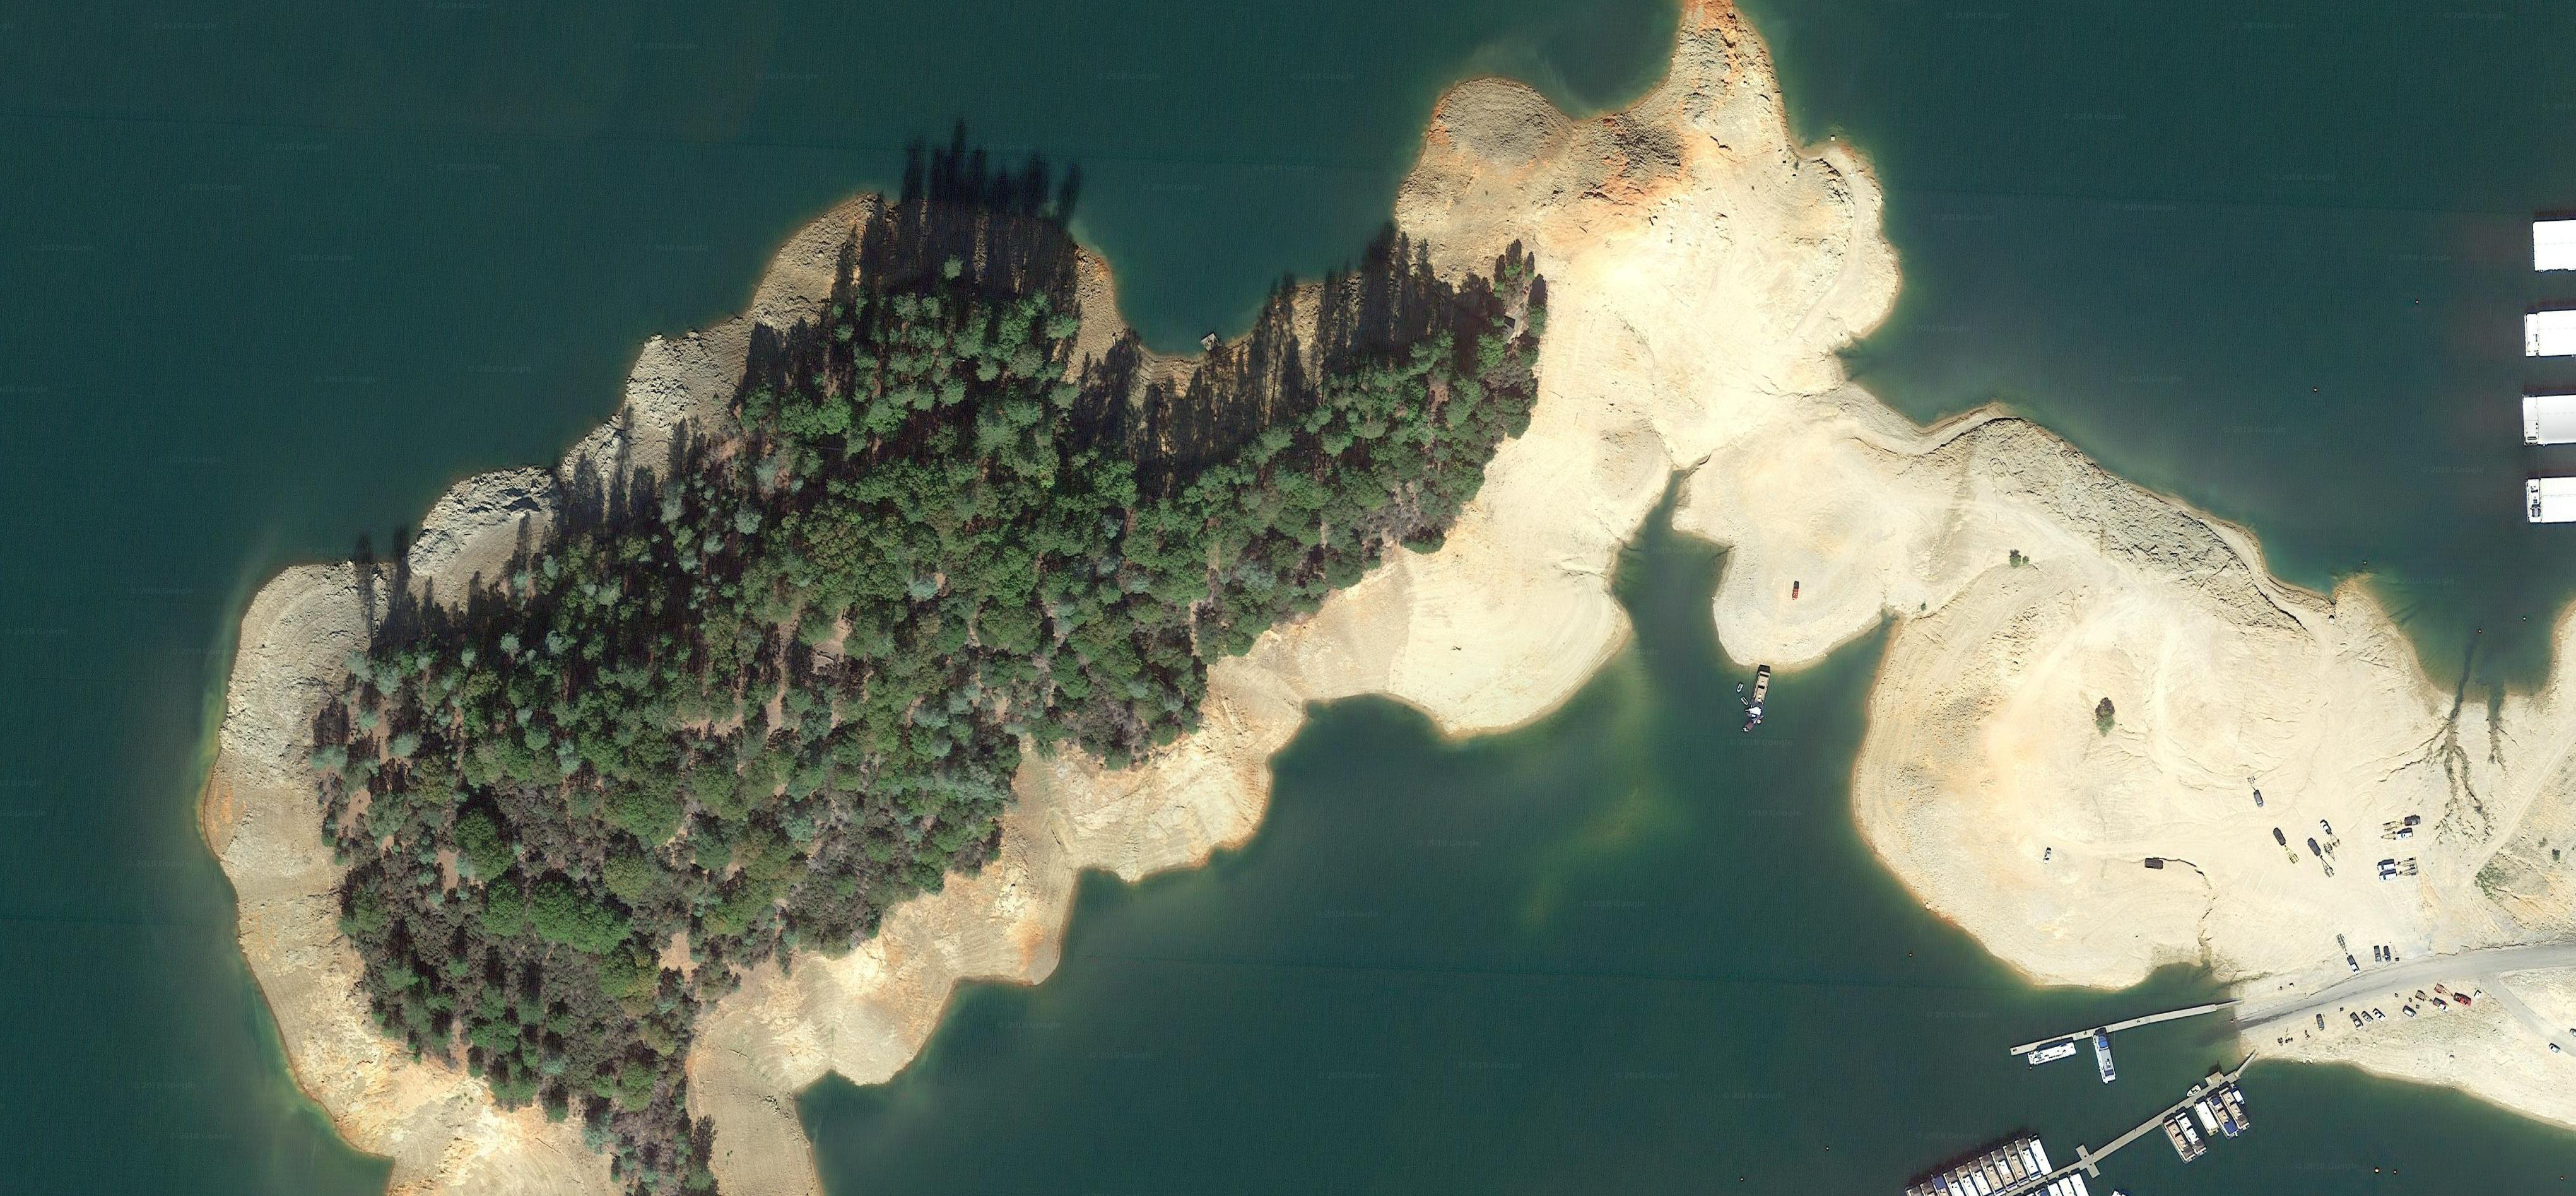
\includegraphics[width=\linewidth]{./media/images/fg_sat_map}
  \tiny{\textit{FlightGear's map server is fast and provides detail down to the
      individual tree level (Photo:
      {\href{http://mpmap02.flightgear.org/}{flightgear map server}})}}
  }
A mapping tool based on FlightGear's data may be had with
\href{http://wiki.flightgear.org/Atlas}{\textsc{atlas}}. You define the area
and features that you want to map and Atlas provides a nice shaded relief map. 

Other sources for map inspiration include \textsc{qgis} geographical information
system software and \href{http://mpmap02.flightgear.org/}{\textsc{flightgear's map server}}. Both these applications
offer stunningly sharp detail.
\subsection{space simulators}
\marginnote{
  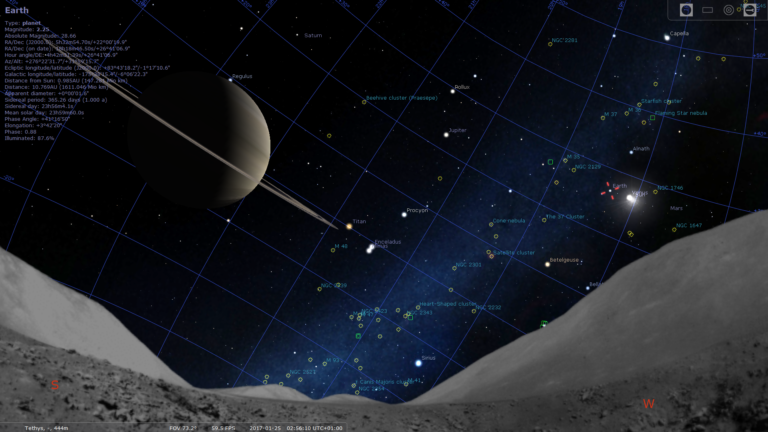
\includegraphics[width=\linewidth]{./media/images/stellarium}
  \tiny{\textsc{Stellarium's views offer} \textit{``world-class'' experiences
      (Photo:
      {\href{https://www.star-watcher.ch/equipment/stellarium-app/}{Karol
          Novotny, star\textemdash watcher}})}}
  }
\noindent Space simulators like \href{https://stellarium.org/}{\textsc{stellarium}} and
\href{https://celestia.space/}{\textsc{celestia}} come as ready\textendash made sources
for star maps and scenery. Both offer the ability to locate yourself in any
number of reference points from which to base your story. Imagine a Science
Fiction story who's view out the ship's portal is an accurate depiction of the
location's celestial bodies!

\section{plotting the story layers}
Works of Interactive Fiction that do not (or at least minimally) commit
\href{http://pdf.textfiles.com/books/iftheorybook.pdf}{\textsc{crimes against mimesis}}
require careful planning. When the reader is rewarded having achieved the next
phase of the story to a beautiful scene including, ``golden, sun\textendash
drenched waves splashing against the towering rock formations,'' the last thing
we want our locutor to experience is this:
\begin{quote}
  Gold Beach
  
  \ldots golden, sun\textendash
  drenched waves splash against the towering rock formations in relief.''

  \textbf{> look at rocks}

  You see no rocks here.
\end{quote}

\noindent Plotting isn't limited to your physical world layer; you can use it to map your plot and narrative layers too.

\begin{figure*}[h]
 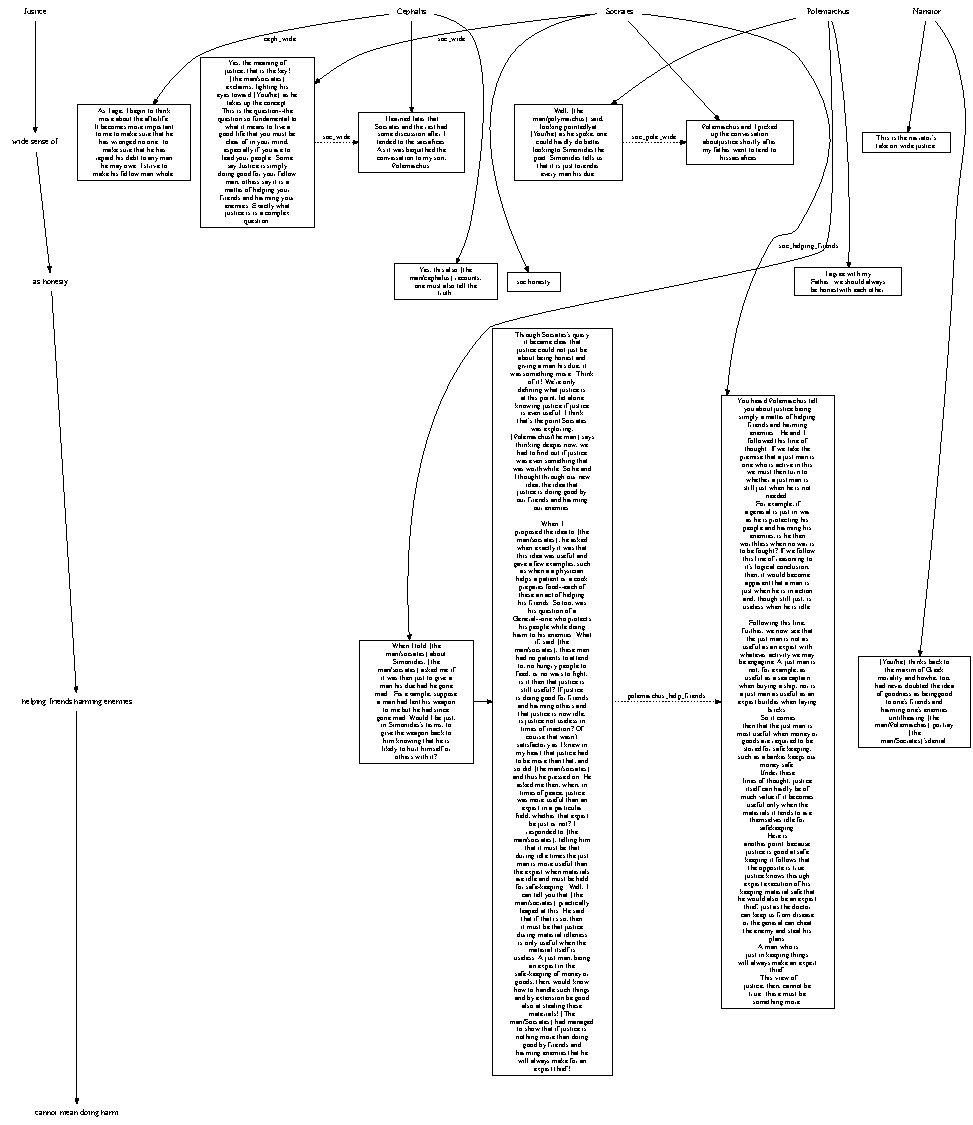
\includegraphics[width=\linewidth]{./media/images/story_board.pdf}%
  \small{\textsc{\\ Creating a story board} goes a long way toward completion
    and enhancing coherence (Photo:
    \href{http://portfolio.cooper.stevenson.name}{\textsc{Cooper Stevenson).}}}
  \label{fig:storyboard}%                                                 
\end{figure*}
For example, in \textsc{\vref{fig:storyboard}} I lay out the the conversation in Plato's
\href{https://www.gutenberg.org/files/1497/1497-h/1497-h.htm}{\textsc{the
    republic}}. Each character is listed horizontally across the top of the plot. Each topic they discuss, in order, is listed vertically along the
left\textendash side. From here we can create \small{\texttt{ask/tell}} directives for
the compiler.


% to generate diagram
% $ dot -Tsvg conv_short.dot -o conv_short.svg
% then convert to PDF
%This didn't scale well but did manage to get in doc:
% $ dot2tex --figonly --graphstyle "scale=0.5" ./conv_short.dot > /home/cstevens/doc/if/dot.tex
\begin{figure*}[h]
 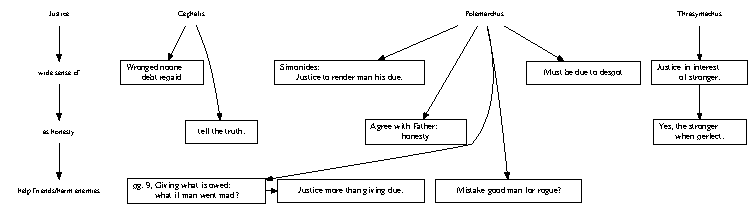
\includegraphics[width=\linewidth]{./media/images/conv_short.pdf}%
  \small{\textsc{\\ Mapping the story}, bit by bit, from source material. This
    simplified view depicts the plotting process; source
    page numbers references are helpful for
    later fleshing out your story. (Photo: \href{http://portfolio.cooper.stevenson.name}{\textsc{Cooper Stevenson}).}}
\end{figure*}

In the next edition of \textit{Discoverer's Digest} I will include the code
snippets for producing the examples of world/plot/narrative plotting I cited
above.

